
%%%%%%%%%%%%%%%%%%%%%%%%%%%%%%%%%%%%%%%%%%%%%%%%%%%%%%%%%%%%%%%%%%%
%%% Documento LaTeX 											%%%
%%%%%%%%%%%%%%%%%%%%%%%%%%%%%%%%%%%%%%%%%%%%%%%%%%%%%%%%%%%%%%%%%%%
% Título:	Plantilla de TFG/TFM
% Autor:  Carlos Andres Goez, Juan Pablo Baena 
% Fecha:  2020-03-12
%%%%%%%%%%%%%%%%%%%%%%%%%%%%%%%%%%%%%%%%%%%%%%%%%%%%%%%%%%%%%%%%%%%
%	Modo:					PDFLaTeX.
%%%%%%%%%%%%%%%%%%%%%%%%%%%%%%%%%%%%%%%%%%%%%%%%%%%%%%%%%%%%%%%%%%%
%------------------------------

\chapterbegin{Desarrollo}
\minitoc

Con el objetivo de simplificar el desarrollo de la máquina esta se dividió en subsistemas para que cada uno es estos cumpla un tarea simple. Los subsistemas en los que se dividió el sistema son:
\begin{itemize}
	\item \textbf{Empacar tallo}
		Ubica el tallo de la flor dentro del capuchon, hasta alcanzar el extremo del capuchon.
	\item \textbf{Empacar botón}
		Situa la porcion faltante de la flor dentro del capuchon 
	\item \textbf{Preparar Capuchon}
		Posiciona el capucho de la flor para que esta sea empacada.
	\item \textbf{Separador por clasificacón}
		Ubica las flores en una diferente salida dependiendo de la clasificación de la misma
	\item \textbf{Clasificación}
		A partir de un algoritmo de procesamiento digital de imágenes clasifica las flores según sea su categoría.
	\item \textbf{Monitorear}
		Almacena los datos de la flor y verifica que no posea cuerpos extraños o enfermedades.
\end{itemize}


\section{Identificación de necesidades }
Como parte del diseño preliminar del proyecto se realizó un matriz de necesidades enfocada en clasificar las necesidades identificadas en la vigilancia tecnológica y la documentación recolectada para realizar el planteamiento del problema y la justificación del proyecto. En esta matriz se pondera cada necesidad por nivel de importancia, se le asignan características generales y se da un estándar de medida.

A continuación se presenta el diagrama general de la solución

\begin{figure}[htb]
	\centering
	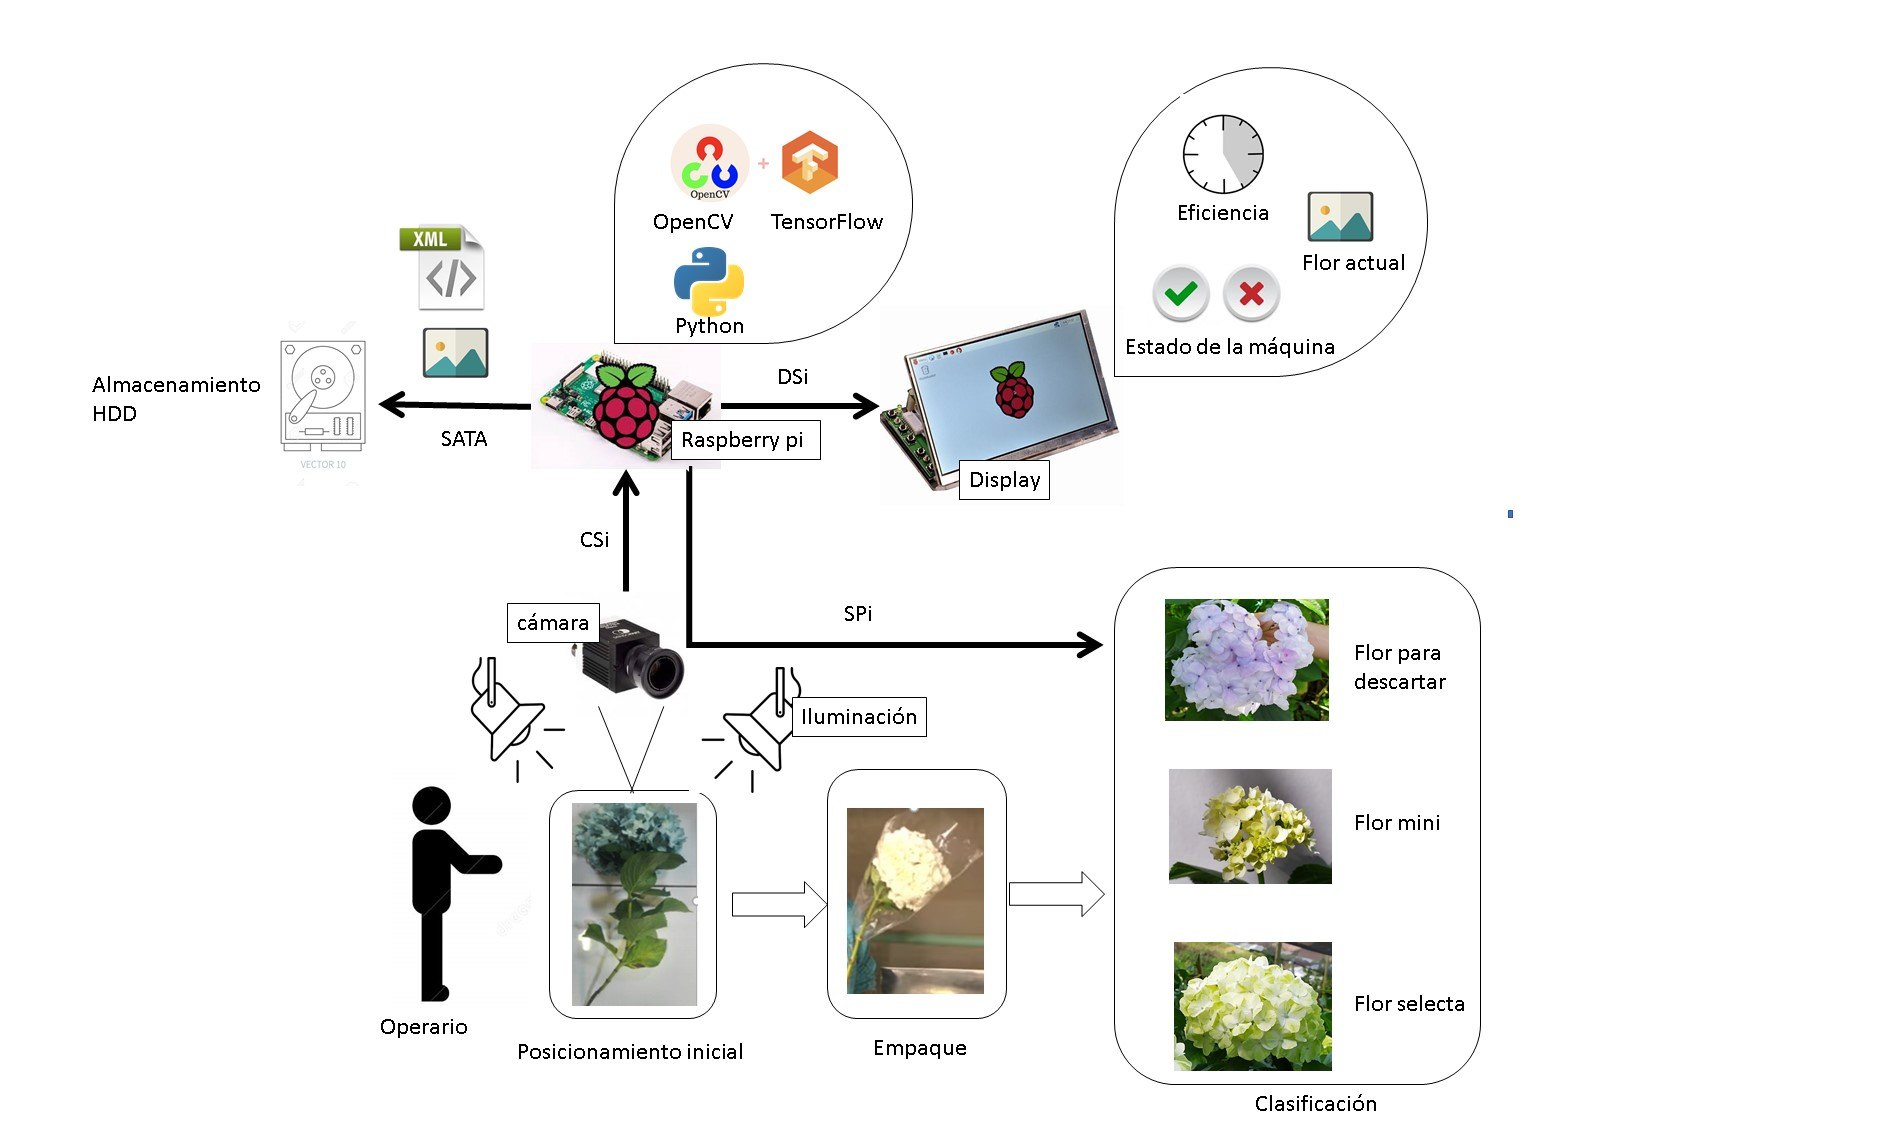
\includegraphics[scale=0.4]{Figuras/Diagrama}
	\caption{Digrama general}
	\label{fig:dGeneral}
\end{figure}


% Table generated by Excel2LaTeX from sheet 'Hoja1'
\begin{table}[H]
	\centering
	\caption{Matriz Necesidades}
	\scalebox{0.9}{
	\begin{tabular}{lp{14.07em}cp{19.855em}p{5.355em}}
		\hline
		\multicolumn{1}{p{2.785em}}{\textbf{\#}} & \textbf{Necesidad} & \multicolumn{1}{p{6em}}{\textbf{Importancia}} & \textbf{Característica} & \textbf{Medida} \\
		\hline
		1  & Reducir tiempos de la postcosecha\newline{} & 5  & Velocidad de operaciones de clasificación empaque y monitoreo & Unidades min \\
		2  & Reducir costo de operación\newline{} & 4  & Costo de postcosecha & COP \\
		3  & Capacidad de los operarios de interactuar con la máquina\newline{} & 3  & Facilidad de operación & Subjetivo \\
		4  & Procesamiento de imágenes\newline{} & 4  & Confiabilidad & \% \\
		5  & Vida Util\newline{} & 3  & Duración del equipo en funcionamiento & Años \\
		\hline
	\end{tabular}}%
	\label{tab:addlabel}%
\end{table}%

Como resultado de la matriz de necesidades se concluye que reducir los tiempos de la postcosecha es el punto más importante solucionar, esto conlleva consigo también una reducción de costos en la operación y que el sistema sea lo suficiente mente confiable para las operaciones que realiza.

\section{Diseño de concepto}
Luego de tener claridad sobre las diferentes necesidades que pretende desarrollar el
proyecto y de haber caracterizado las tareas que realizara la máquina, se procedió a
realizar una diagrama general del sistema, este método permite visualizar el sistema a desarrollar de una
manera sencilla, contemplando únicamente entradas y salidas del sistema.
\begin{figure}[H]
	\centering
	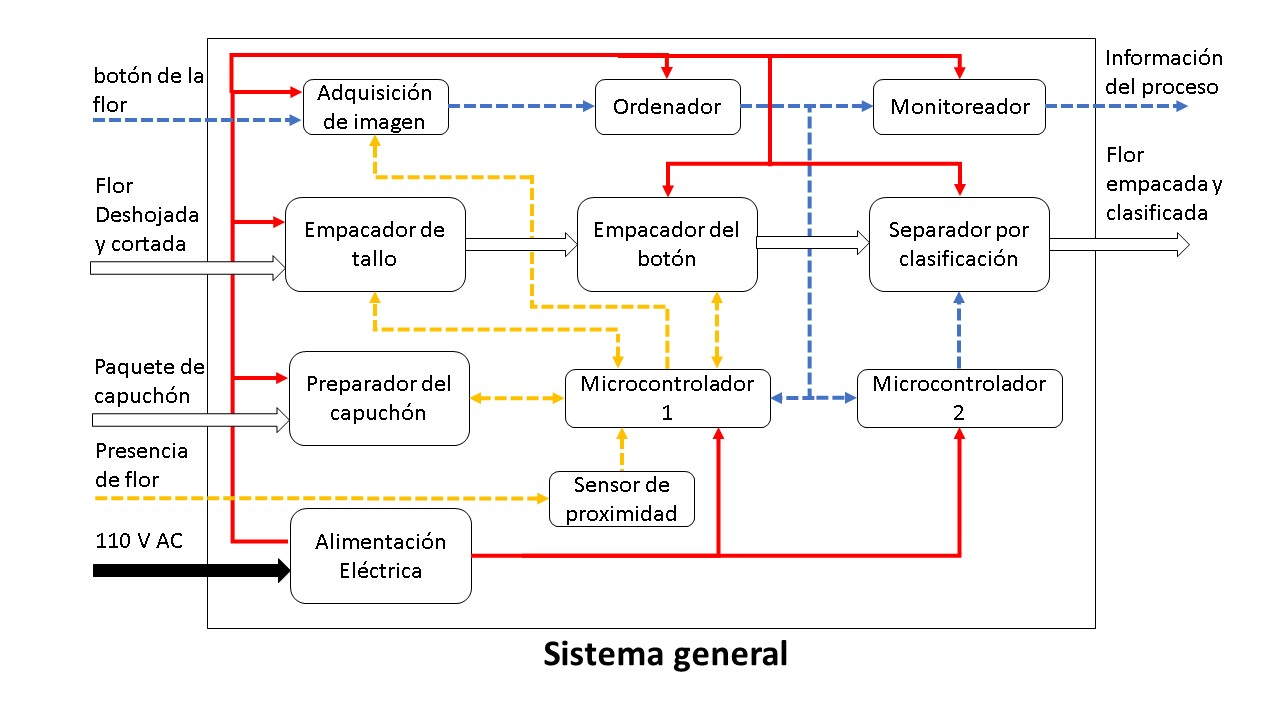
\includegraphics[scale=0.5]{Figuras/SistemaGeneral}
	\caption{Digrama general del sistema}
	\label{fig:dGeneral}
\end{figure}

\subsection{Matriz morfológica}
Para continuar con el diseño de concepto se construye una matriz con las tecnologías
reportadas en cada registro de soluciones, para las diferentes funciones del dispositivo, y
se trazan rutas que definen los componentes que conforman los conceptos preliminares.
\begin{figure}[H]
	\centering
	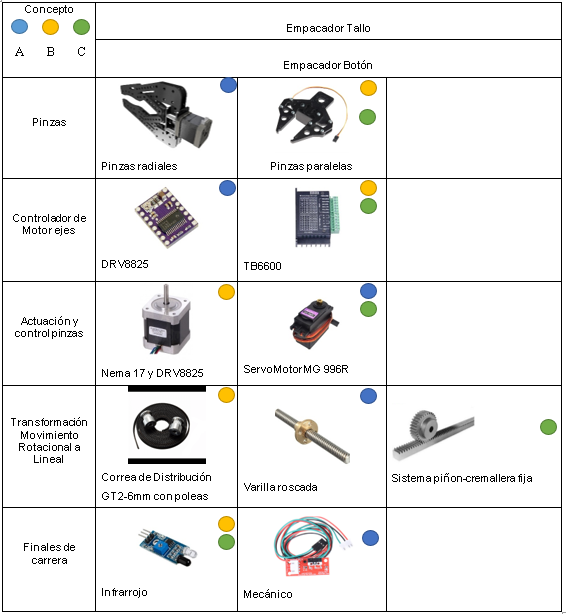
\includegraphics{Figuras/Empacador}
	\caption{Matriz morfologica de subsistemas de empaque tallo y botón}
	\label{fig:MMEmpaque}
\end{figure}
Esta etapas dos etapas se encargan de realizar el empaque de la flor en el capuchón, la primera de ellas el empacador de tallo introduce la flor parcialmente hasta alcanzar el otro extremo del capuchón, donde la segunda etapa el empacador de botón se encarga de finalizar el empacado de la flor introduciendo el botón dentro del capuchón 
\begin{itemize}
	\item \textbf{Concepto A}\\
	Contempla el uso de servo motores, pinzas paralelas, finales de carrera de accionamiento mecánico y un tornillo de bolas para el desplazamiento longitudinal, esta opción es la mejor si se busca suavidad en los movimientos, también requiere poco mantenimiento, pero es la como desventaja tiene que es la más cara, también la integración entre sus componente no es la mejor de las opciones.
	\item \textbf{Concepto B}\\
	Esta opción utiliza motore paso a paso, con pinzas radiales y desplazamiento por medio de una correa de distribución, destaca por su bajo precio, poco mantenimiento y disponibilidad de las piezas, como desventaja tienen que algunas de sus piezas nos son duraderas por lo que se deben cambiar con regularidad
	\item \textbf{Concepto C}\\
	Esta opción es una combinación de las dos anteriores con la diferencia del desplazmiento que se realiza con un piñon cremallera,se caracteriza por su poco mantenimiento y confiabilidad pero su precio es su principal desventaja
\end{itemize}



\begin{figure}[H]
	\centering
	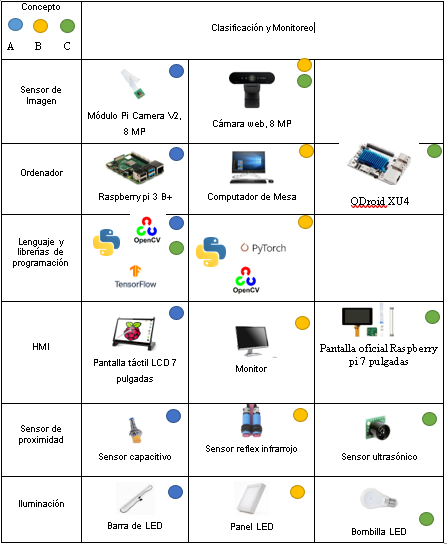
\includegraphics{Figuras/Matriz_Clasificacion}
	\caption{Matriz morfologica de subsistemas de clasificación y monitoreo}
	\label{fig:MMClasificación}
\end{figure}
Esta etapas se hacen cargo de la clasificación y monitoreo de la flor, para realizar utilizan ordenadores camaras y un sistema de iluminación para garantizar 

\begin{itemize}
	\item \textbf{Concepto A}\\
	Esta opcion se caracteriza por su portabilidad y integración entre componentes ya que tanto ordenador, como camara y pantalla son de la plataforma Pi, encuanto a software cuenta como desventaja tiene su limitado poder de procesamiento
	\item \textbf{Concepto B}\\
	Utiliza un ordenador de mesa os cual le otorga  un poder de procesamiento superior a los otros conceptos,como desventaja tiene su baja portabilidad y la calidad de imagenes que puede capturar.
	\item \textbf{Concepto C}\\
	Esta opcion es muy economia debido a su uso de componentes de bajo costo como su ordenador Droid pero tambien la integración entre sus componentes es complicada y la calidad de sus imagenes tambien es inferior a los otros conceptos.
\end{itemize}

\begin{figure}[H]
	\centering
	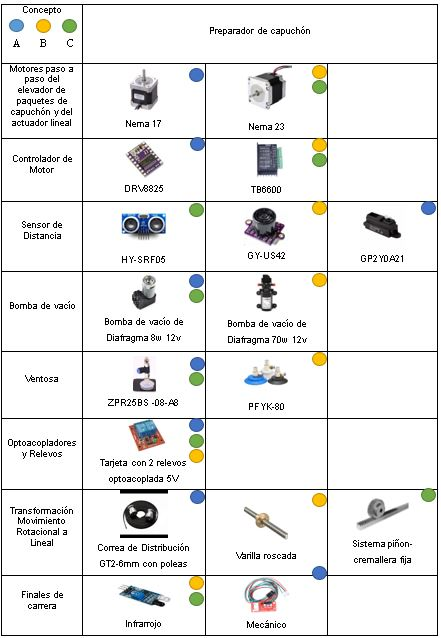
\includegraphics{Figuras/MMCapuchon}
	\caption{Matriz morfologica de subsistema de preparación capuchon}
	\label{fig:MMCapuchon}
\end{figure}
Esta es la primera etapa que controla que microcontrolador 1 y la primera tambíen del ciclo de tareas de todo el sistema. Este subsistema se encarga de preparar/abrir el capuchón en el cúal se insertará posteriormente la flor. Esta función la cumple por medio de un actuador lineal accionado por un motor paso a paso que en su punta posee una ventosa que recibe presión negativa de una bomba de vacío para sujetar un lado del capuchón que finalmente se abre completamente por la fuerza gravitatoria. Estos capuchones son a su vez posicionados para su sujetación a través de un elevador de los paquetes de capuchón que compensa la altura respecto al punto de sujeción a medida que los capuchónes individuales van siendo utilizados, este proceso se efectúa mediante un motor paso a paso que su actuación depende de la altura medida por un sensor de distancia. 
\begin{itemize}
	\item \textbf{Concepto A}\\
	Contempla el uso del motor NEMA 17 para el actuador lineal y del elevador junto con un controlador de corriente pico máxima 2.5 A, un sensor de distancia análogo tipo SHARP con el rango justo para la aplicación, bomba de vacío de 8w, ventosa de fuelle de 25mm, movimiento lineal efectuado por correas de distribución y finales de carrera mecánicos. Esta opción tiene como ventaja más notoria la reducción de precios frente a las otras opciones debido a que se utilizan los elementos más ajustados posibles con elementos comerciales a las especificaciones requeridas pero sacrificando velocidad de actuación debido al motor de menor capacidad. 
	\item \textbf{Concepto B}\\
	Contempla el uso del motor NEMA 23 para el actuador lineal y del elevador junto con un controlador de corriente pico máxima 5 A, un sensor de distancia ultrasónico con rango 20 a 720 cm, bomba de vacío de 8w, ventosa de fuelle de 25mm, movimiento lineal efectuado por Varillas roscadas y finales de carrera reflex infrarojo. Esta opción tiene como ventaja un actuación más rápida respecto a la primera opción, sin embargo, con elementos más costos y con menos precisión en la medición de la altura respecto a la opción anterior, ya que el sensor ultrasónico tiene una resolución de 1cm. 
	\item \textbf{Concepto C}\\
	Contempla el uso del motor NEMA 23 para el actuador lineal y del elevador junto con un controlador de corriente pico máxima 5 A, un sensor de distancia ultrasónico con rango 2 a 450 cm, bomba de vacío de 70w, ventosa de fuelle de 80mm, movimiento lineal efectuado por un sistema piñon-cremallera y finales de carrera reflex infrarojo. Esta opción tiene como ventaja la actuación más rápida respecto a las otras opciones, sin embargo, con los elementos más costos de las opciones en la actuación, además, con la desventaja de que el sistema piñon-cremallera se debería fabricar. En la medición de la altura se contempla uno de los sensores más economicos del mercado y con una resolución de 0.3cm que se encuentra dentro del rango de tolerancia en la medición de distancia. 
\end{itemize}
\begin{figure}[H]
	\centering
	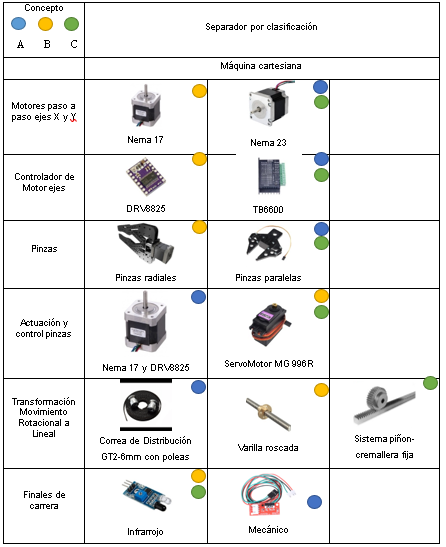
\includegraphics{Figuras/MatrizCartesiana}
	\caption{Matriz morfologica de subsistema de separación por clasificación}
	\label{fig:Cartesiana}
\end{figure}
Esta subsistema la controla el microcontrolador 2 y es la última del ciclo de tareas de todo el sistema. Este subsistema se encarga de clasificar físicamente las flores ingresadas al sistema mediante una máquina cartensiana 2 ejes que sujeta la flor por medio pinzas y las ubica en la base deslizante correspondiente según la clasificación recibida por el ordenador principal.  
\begin{itemize}
	
	\item \textbf{Concepto A}\\
	Contempla el uso del motor NEMA 23 para los dos ejes de movimiento de la máquina cartesiana con movimiento lineal por correas de distribución y poleas. Pinzas paralelas actuadas por un NEMA 17 y su controlador de 2.5 A pico junto con finales de carrera mecánicos. Destaca esta opción por ser la mejor en precio-calidad, con la mayor velocidad de actuación de las opciones consideradas, además del mejor agarre en las pinzas por ser de tipo paralelas y con el NEMA 17. 
	\item \textbf{Concepto B}\\
	Contempla el uso del motor NEMA 17 para los dos ejes de movimiento de la máquina cartesiana con movimiento lineal por varilla roscada. Pinzas radiales actuadas por el ServoMotor MG 996R junto con finales de carrera réflex infrarrojos. Es la opción con menor costo, sin embargo, con una actuación lenta debido a la menor capacidad del motor de los ejes respecto las demás.
	\item \textbf{Concepto C}\\
	Contempla el uso del motor NEMA 23 para los dos ejes de movimiento de la máquina cartesiana con movimiento lineal por un sistema piñon-cremallera. Pinzas paralelas actuadas por el ServoMotor MG 996R junto con finales de carrera réflex infrarrojos. Es una opción con la desventaja de que el sistema piñon-cremallera se debería fabricar, sin embargo, posee una buena velocidad de actuación. 
\end{itemize}

\subsection{Selección de concepto}
Con el objetivo de seleccionar el concepto que permita desarrollar el proyecto de la mejor
manera y obtener los mejores resultados, se utiliza una matriz de decisión, en la que se
especifican diferentes criterios de decisión y su peso, se le da una calificación a cada 
La información presentada en este documento es de exclusiva responsabilidad de los autores y no
compromete a la EIA.
concepto sobre el criterio y se saca un ponderado, al final, el criterio con mayor puntaje en
la suma de los ponderados será el elegido para desarrollar el proyecto.
% Table generated by Excel2LaTeX from sheet 'Hoja1'
\begin{table}[H]
	\centering
	\caption{Matriz de desición Empacador Flor}
	\scalebox{0.9}{
	\begin{tabular}{p{5.355em}cp{5.355em}cp{5.355em}cp{5.355em}c}
		\hline
		\multicolumn{8}{p{42.84em}}{\textbf{Empacador Flor}}
		\\
		\hline
		\multicolumn{2}{c}{} &
		\multicolumn{2}{p{10.71em}}{\textbf{Concepto A}} &
		\multicolumn{2}{p{10.71em}}{\textbf{Concepto B}} &
		\multicolumn{2}{p{10.71em}}{\textbf{Concepto C}}
		\\
		\hline
		\textbf{Criterio de decisión} &
		\multicolumn{1}{p{5.355em}}{\textbf{Peso}} &
		\textbf{C} &
		\multicolumn{1}{p{5.355em}}{\textbf{P}} &
		\textbf{C} &
		\multicolumn{1}{p{5.355em}}{\textbf{P}} &
		\textbf{C} &
		\multicolumn{1}{p{5.355em}}{\textbf{P}}
		\\
		Costos &
		30\% &
	\multicolumn{1}{c}{3} &
		0,9 &
		\multicolumn{1}{c}{4} &
		1,2 &
		\multicolumn{1}{c}{2} &
		0,6
		\\
		Integración entre componentes &
		20\% &
		\multicolumn{1}{c}{4} &
		0,8 &
		\multicolumn{1}{c}{4} &
		0,8 &
		\multicolumn{1}{c}{3} &
		0,6
		\\
		Presición en Posicionamiento &
		10\% &
		\multicolumn{1}{c}{5} &
		0,5 &
		\multicolumn{1}{c}{4} &
		0,4 &
		\multicolumn{1}{c}{3} &
		0,3
		\\
		Suavidad de movimiento &
		5\% &
		\multicolumn{1}{c}{4} &
		0,2 &
		\multicolumn{1}{c}{4} &
		0,2 &
		\multicolumn{1}{c}{3} &
		0,15
		\\
		Disponibilidad &
		15\% &
		\multicolumn{1}{c}{3} &
		0,45 &
		\multicolumn{1}{c}{4} &
		0,6 &
		\multicolumn{1}{c}{3} &
		0,45
		\\
		Facilidad de instalación &
		10\% &
		\multicolumn{1}{c}{3} &
		0,3 &
		\multicolumn{1}{c}{4} &
		0,4 &
		\multicolumn{1}{c}{3} &
		0,3
		\\
		Mantenimiento &
		10\% &
		\multicolumn{1}{c}{3} &
		0,3 &
		\multicolumn{1}{c}{4} &
		0,4 &
		\multicolumn{1}{c}{4} &
		0,4
		\\
		Total &
		&
		\multicolumn{2}{c}{3,45} &
		\multicolumn{2}{c}{4} &
		\multicolumn{2}{c}{2,8}
		\\
		Posición &
		&
		\multicolumn{2}{c}{1} &
		\multicolumn{2}{c}{2} &
		\multicolumn{2}{c}{3}
		\\
		\hline
		\textbf{Desarrollar} &
		&
		\multicolumn{2}{p{10.71em}}{\textbf{SI}} &
		\multicolumn{2}{p{10.71em}}{\textbf{NO}} &
		\multicolumn{2}{p{10.71em}}{\textbf{NO}}
		\\
		\hline
	\end{tabular}}%
	\label{tab:addlabel}%
\end{table}%

% Table generated by Excel2LaTeX from sheet 'Hoja4'
\begin{table}[H]
	\centering
	\caption{Matriz de decisión Clasificador y Monitoreador}
	\scalebox{0.9}{
	\begin{tabular}{p{5.355em}cp{5.355em}cp{5.355em}cp{5.355em}c}
		\hline
		\multicolumn{8}{p{42.84em}}{\textbf{Clasificador y Monitoreador}}
	\\
		\hline
		\multicolumn{2}{c}{} &
		\multicolumn{2}{p{10.71em}}{\textbf{Concepto A}} &
		\multicolumn{2}{p{10.71em}}{\textbf{Concepto B}} &
		\multicolumn{2}{p{10.71em}}{\textbf{Concepto C}}
	\\
		\hline
		\textbf{Criterio de decisión} &
		\multicolumn{1}{p{5.355em}}{\textbf{Peso}} &
		\textbf{C} &
		\multicolumn{1}{p{5.355em}}{\textbf{P}} &
		\textbf{C} &
		\multicolumn{1}{p{5.355em}}{\textbf{P}} &
		\textbf{C} &
		\multicolumn{1}{p{5.355em}}{\textbf{P}}
		\\
		Costos &
		30\% &
		\multicolumn{1}{c}{5} &
		2 &
		\multicolumn{1}{c}{3} &
		1 &
		\multicolumn{1}{c}{4} &
		1,2
		\\
		Integración entre componentes &
		10\% &
		\multicolumn{1}{c}{4} &
		0,4 &
		\multicolumn{1}{c}{4} &
		0,4 &
		\multicolumn{1}{c}{3} &
		0,3
		\\
		Capacidad de procesamiento &
		20\% &
		\multicolumn{1}{c}{3} &
		0,6 &
		\multicolumn{1}{c}{4} &
		0,8 &
		\multicolumn{1}{c}{3} &
		0,6
		\\
		Capacidad de adaptación en clasificación &
		10\% &
		\multicolumn{1}{c}{4} &
		0,4 &
		\multicolumn{1}{c}{4} &
		0,4 &
		\multicolumn{1}{c}{3} &
		0,3
		\\
		Calidad Imágenes &
		10\% &
		\multicolumn{1}{c}{3} &
		0,3 &
		\multicolumn{1}{c}{2} &
		0,2 &
		\multicolumn{1}{c}{2} &
		0,2
		\\
		Disponibilidad &
		10\% &
		\multicolumn{1}{c}{5} &
		0,5 &
		\multicolumn{1}{c}{4} &
		0,4 &
		\multicolumn{1}{c}{3} &
		0,3
		\\
		Facilidad de utilización &
		5\% &
		\multicolumn{1}{c}{4} &
		0,2 &
		\multicolumn{1}{c}{4} &
		0,2 &
		\multicolumn{1}{c}{3} &
		0,15
		\\
		Facilidad de visualización &
		5\% &
		\multicolumn{1}{c}{4} &
		0,2 &
		\multicolumn{1}{c}{4} &
		0,2 &
		\multicolumn{1}{c}{4} &
		0,2
		\\
		Total &
		&
		\multicolumn{1}{c}{4,6} &
		&
		\multicolumn{1}{c}{3,6} &
		&
		\multicolumn{1}{c}{3,25} &
		
		\\
		Posición &
		&
		\multicolumn{1}{c}{1} &
		&
		\multicolumn{1}{c}{2} &
		&
		\multicolumn{1}{c}{3} &
		
		\\
		\hline
		\textbf{Desarrollar} &
		&
		\textbf{SI} &
		&
		\textbf{NO} &
		&
		\textbf{NO} &
		
		\\
		\hline
	\end{tabular}}%
	\label{tab:addlabel}%
\end{table}%

% Table generated by Excel2LaTeX from sheet 'Hoja2'
\begin{table}[H]
	\centering
	\caption{Matriz de decisión Preparador de capuchón}
	\scalebox{0.9}{
	\begin{tabular}{p{5.785em}cp{5.355em}cp{5.355em}cp{5.355em}c}
		\hline
		\multicolumn{8}{p{43.27em}}{\textbf{Preparador de capuchón}}
		\\
		\hline
		\multicolumn{2}{c}{} &
		\multicolumn{2}{p{10.71em}}{\textbf{Concepto A}} &
		\multicolumn{2}{p{10.71em}}{\textbf{Concepto B}} &
		\multicolumn{2}{p{10.71em}}{\textbf{Concepto C}}
		\\
		\hline
		\textbf{Criterio de decisión} &
		\multicolumn{1}{p{5.355em}}{\textbf{Peso}} &
		\textbf{C} &
		\multicolumn{1}{p{5.355em}}{\textbf{P}} &
		\textbf{C} &
		\multicolumn{1}{p{5.355em}}{\textbf{P}} &
		\textbf{C} &
		\multicolumn{1}{p{5.355em}}{\textbf{P}}
		\\
		Costos &
		40\% &
		\multicolumn{1}{c}{5} &
		2 &
		\multicolumn{1}{c}{3} &
		1,2 &
		\multicolumn{1}{c}{2} &
		0,8
		\\
		Integración entre componentes &
		10\% &
		\multicolumn{1}{c}{4} &
		0,4 &
		\multicolumn{1}{c}{4} &
		0,4 &
		\multicolumn{1}{c}{3} &
		0,3
		\\
		Velocidad de actuación &
		30\% &
		\multicolumn{1}{c}{3} &
		0,9 &
		\multicolumn{1}{c}{5} &
		1,5 &
		\multicolumn{1}{c}{5} &
		1,5
		\\
		Disponibilidad &
		10\% &
		\multicolumn{1}{c}{5} &
		0,5 &
		\multicolumn{1}{c}{5} &
		0,5 &
		\multicolumn{1}{c}{3} &
		0,3
		\\
		Facilidad de montaje &
		5\% &
		\multicolumn{1}{c}{4} &
		0,2 &
		\multicolumn{1}{c}{4} &
		0,2 &
		\multicolumn{1}{c}{3} &
		0,15
		\\
		Facilidad de detección de fallas &
		5\% &
		\multicolumn{1}{c}{4} &
		0,2 &
		\multicolumn{1}{c}{3} &
		0,15 &
		\multicolumn{1}{c}{4} &
		0,2
		\\
		Total &
		100\% &
		\multicolumn{2}{c}{4,2} &
		\multicolumn{2}{c}{3,95} &
		\multicolumn{2}{c}{3,25}
		\\
		Posición &
		&
		\multicolumn{2}{c}{1} &
		\multicolumn{2}{c}{2} &
		\multicolumn{2}{c}{3}
		\\
		\hline
		\textbf{Desarrollar} &
		&
		\multicolumn{2}{p{10.71em}}{\textbf{SI}} &
		\multicolumn{2}{p{10.71em}}{\textbf{NO}} &
		\multicolumn{2}{p{10.71em}}{\textbf{NO}}
		\\
		\hline
	\end{tabular}}%
	\label{tab:addlabel}%
\end{table}%

% Table generated by Excel2LaTeX from sheet 'Hoja2'
\begin{table}[H]
	\centering
	\caption{Matriz de desición Separador por clasificación}
	\scalebox{0.9}{
	\begin{tabular}{p{5.785em}cp{5.355em}cp{5.355em}cp{5.355em}c}
		\hline
		\multicolumn{8}{p{43.27em}}{\textbf{Separador por clasificación}}
		\\
		\hline
		\multicolumn{2}{c}{} &
		\multicolumn{2}{p{10.71em}}{\textbf{Concepto A}} &
		\multicolumn{2}{p{10.71em}}{\textbf{Concepto B}} &
		\multicolumn{2}{p{10.71em}}{\textbf{Concepto C}}
		\\
		\hline
		\textbf{Criterio de decisión} &
		\multicolumn{1}{p{5.355em}}{\textbf{Peso}} &
		\textbf{C} &
		\multicolumn{1}{p{5.355em}}{\textbf{P}} &
		\textbf{C} &
		\multicolumn{1}{p{5.355em}}{\textbf{P}} &
		\textbf{C} &
		\multicolumn{1}{p{5.355em}}{\textbf{P}}
		\\
		Costos &
		30\% &
		\multicolumn{1}{c}{4} &
		1,2 &
		\multicolumn{1}{c}{3} &
		0,9 &
		\multicolumn{1}{c}{5} &
		1,5
		\\
		Integración entre componentes &
		10\% &
		\multicolumn{1}{c}{4} &
		0,4 &
		\multicolumn{1}{c}{4} &
		0,4 &
		\multicolumn{1}{c}{3} &
		0,3
		\\
		Velocidad de actuación &
		40\% &
		\multicolumn{1}{c}{5} &
		2 &
		\multicolumn{1}{c}{3} &
		1,2 &
		\multicolumn{1}{c}{4} &
		1,6
		\\
		Disponibilidad &
		10\% &
		\multicolumn{1}{c}{5} &
		0,5 &
		\multicolumn{1}{c}{5} &
		0,5 &
		\multicolumn{1}{c}{3} &
		0,3
		\\
		Facilidad de montaje &
		5\% &
		\multicolumn{1}{c}{4} &
		0,2 &
		\multicolumn{1}{c}{4} &
		0,2 &
		\multicolumn{1}{c}{3} &
		0,15
		\\
		Facilidad de detección de fallas &
		5\% &
		\multicolumn{1}{c}{4} &
		0,2 &
		\multicolumn{1}{c}{3} &
		0,15 &
		\multicolumn{1}{c}{3} &
		0,15
		\\
		Total &
		100\% &
		\multicolumn{2}{c}{4,5} &
		\multicolumn{2}{c}{3,35} &
		\multicolumn{2}{c}{4}
		\\
		Posición &
		&
		\multicolumn{2}{c}{1} &
		\multicolumn{2}{c}{2} &
		\multicolumn{2}{c}{3}
		\\
		\hline
		\textbf{Desarrollar} &
		&
		\multicolumn{2}{p{10.71em}}{\textbf{SI}} &
		\multicolumn{2}{p{10.71em}}{\textbf{NO}} &
		\multicolumn{2}{p{10.71em}}{\textbf{NO}}
		\\
		\hline
	\end{tabular}}%
	\label{tab:addlabel}%
\end{table}%



\section{Diagrama de bloques del sistema}
Los diagramas de bloques del sistema permiten ver en profundidad la interacción de cada uno de los componentes, realizar este diagrama permite evaluar los conceptos seleccionados por que en este se observan las integraciones entre componentes por lo que es muy sencillo observar posibles fallos de la solución y dimensionar los componentes a obtener.
\begin{figure}[H]
	\centering
	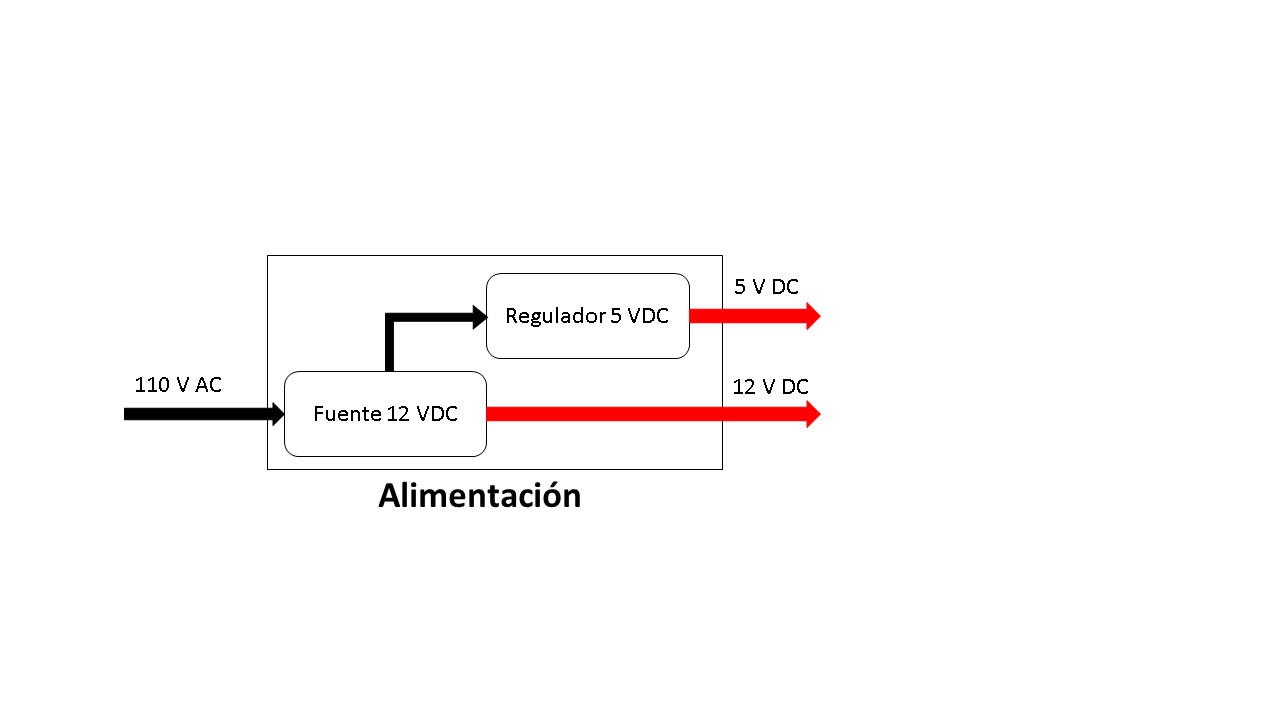
\includegraphics[scale=0.4]{Figuras/Alimentacion}
	\caption{Diagrama de bloques alimentación}
	\label{fig:DBAlimentacion}
\end{figure}

\begin{figure}[htb]
	\centering
	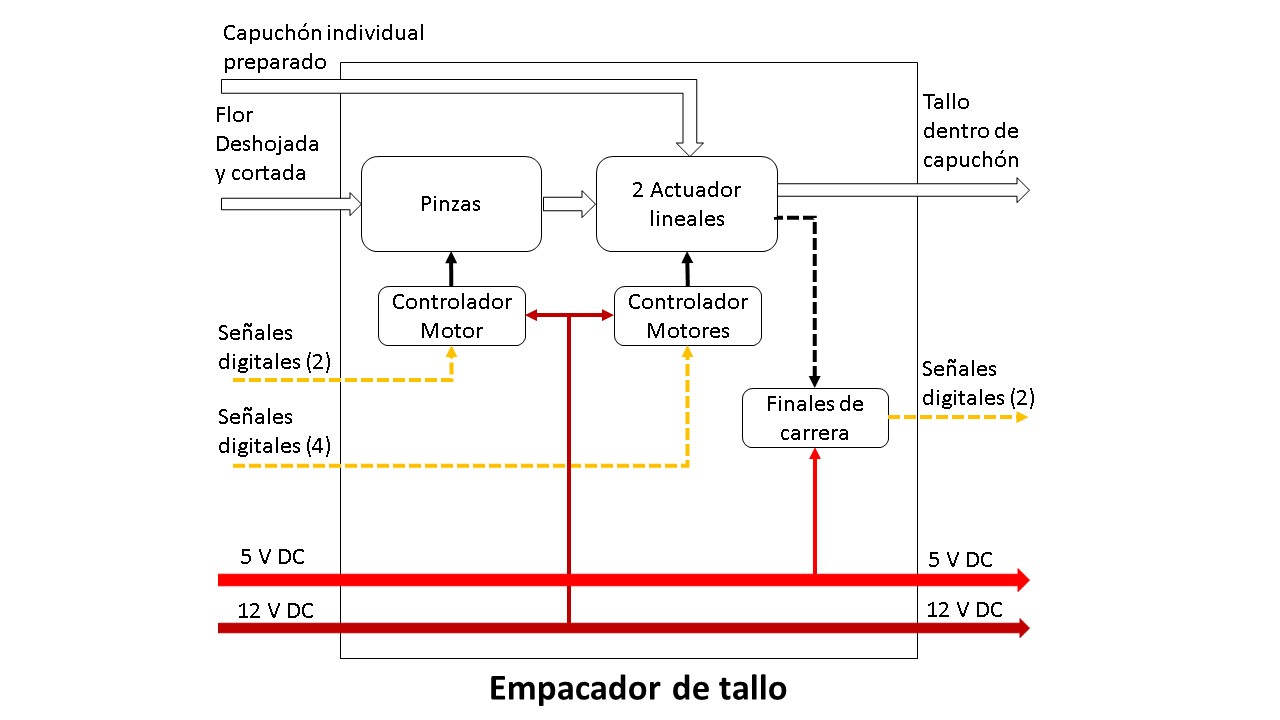
\includegraphics[scale=0.4]{Figuras/PreparadorTallo}
	\caption{Diagrama de bloques empacador de tallo}
	\label{fig:DBAlimentacion}
\end{figure}
\begin{figure}[H]
	\centering
	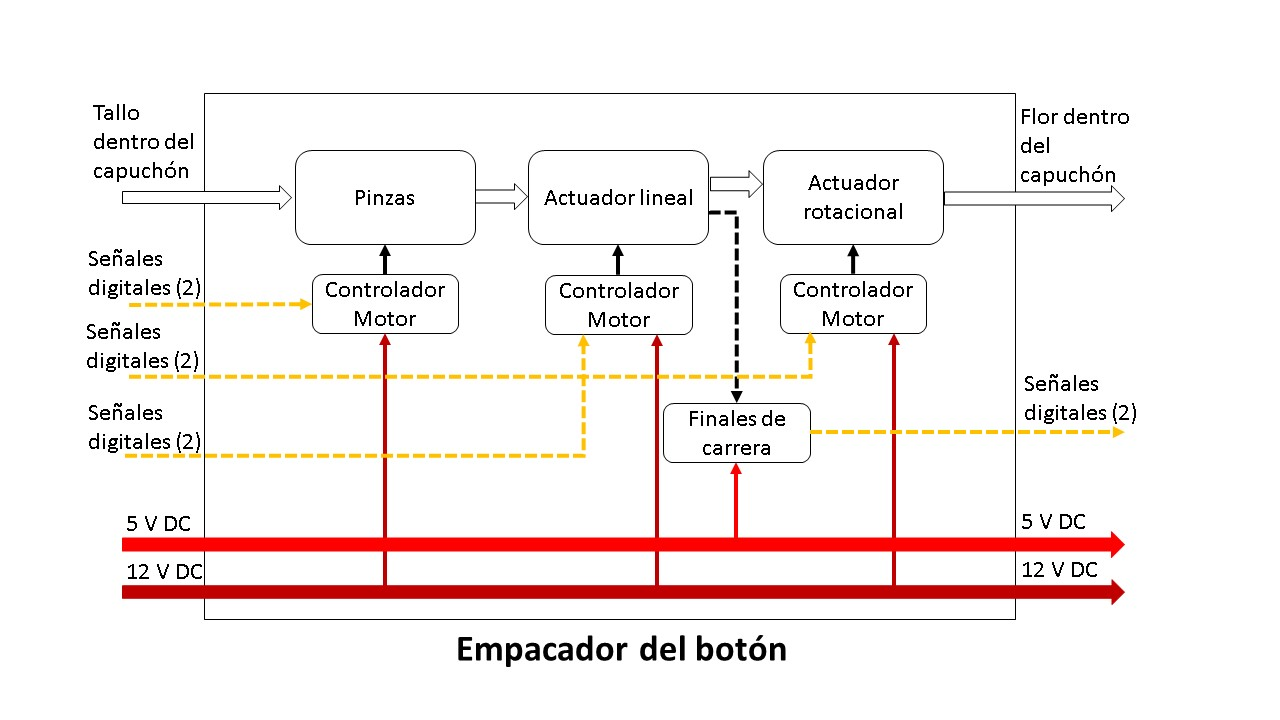
\includegraphics[scale=0.4]{Figuras/EmpacadorBoton}
	\caption{Diagrama de bloques empacador botón}
	\label{fig:DBAlimentacion}
\end{figure}
\begin{figure}[H]
	\centering
	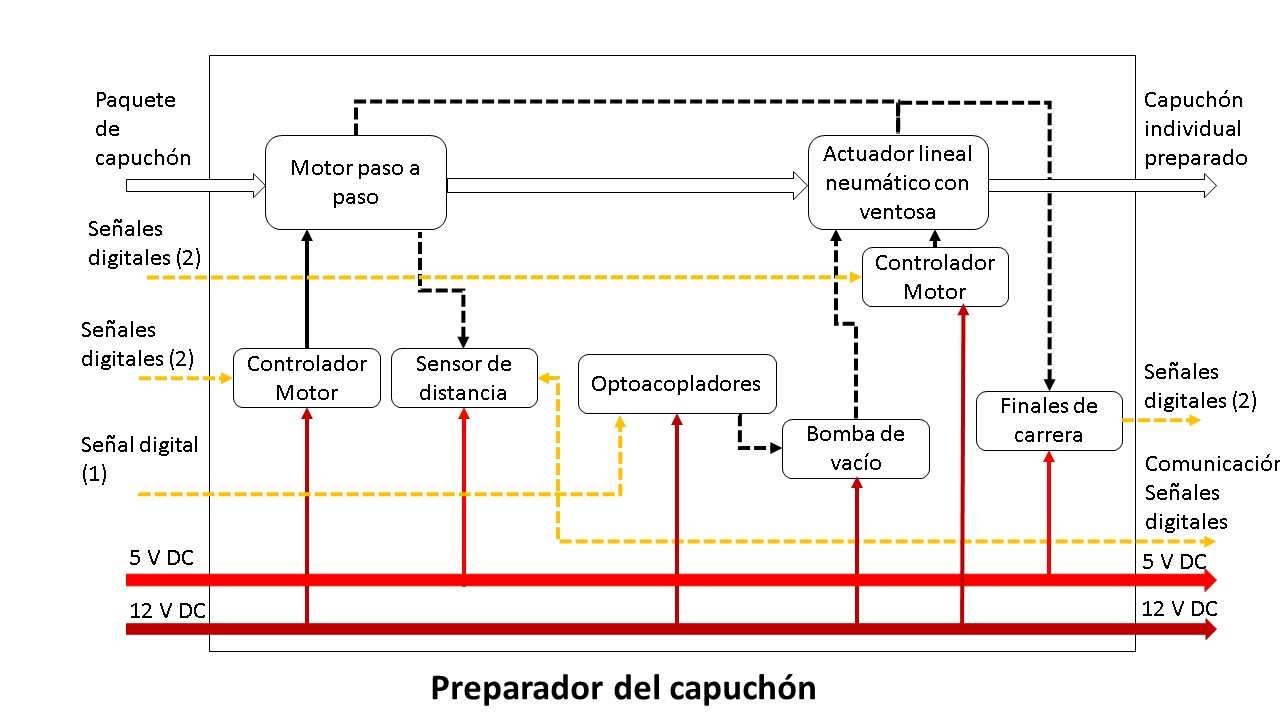
\includegraphics[scale=0.5]{Figuras/PreparadorCapuchon}
	\caption{Diagrama de bloques preparador capuchón}
	\label{fig:DBAlimentacion}
\end{figure}


\begin{figure}[H]
	\centering
	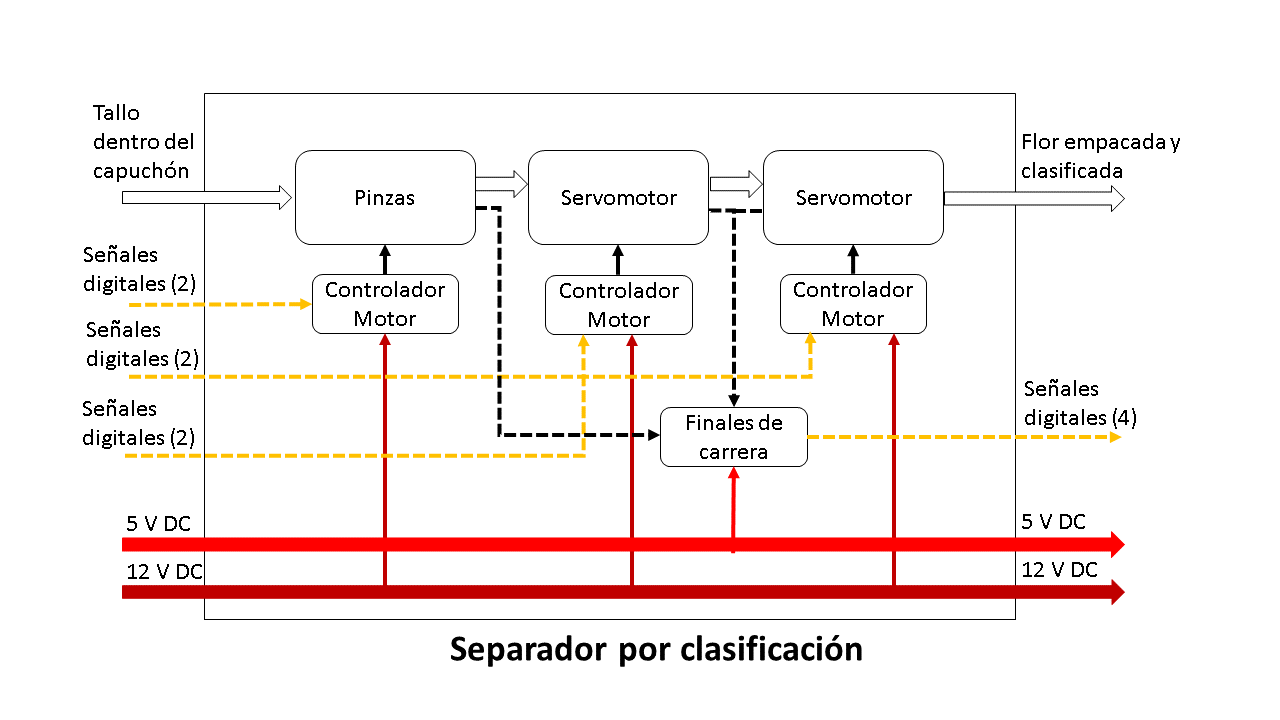
\includegraphics[scale=0.4]{Figuras/SeparadorClasificacion}
	\caption{Diagrama de bloques alimentación}
	\label{fig:DBAlimentacion}
\end{figure}

\begin{figure}[H]
	\centering
	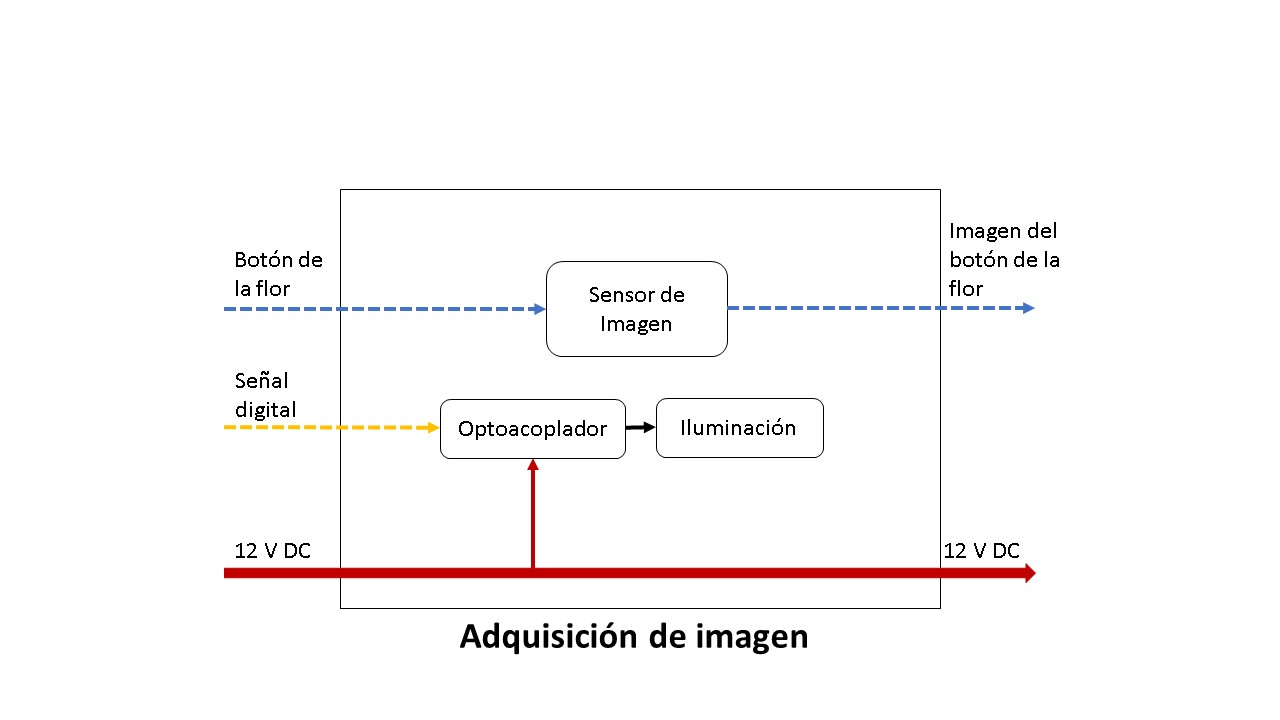
\includegraphics[scale=0.4]{Figuras/AdquisicionImagen}
	\caption{Diagrama de bloques alimentación}
	\label{fig:DBAlimentacion}
\end{figure}

\begin{figure}[H]
	\centering
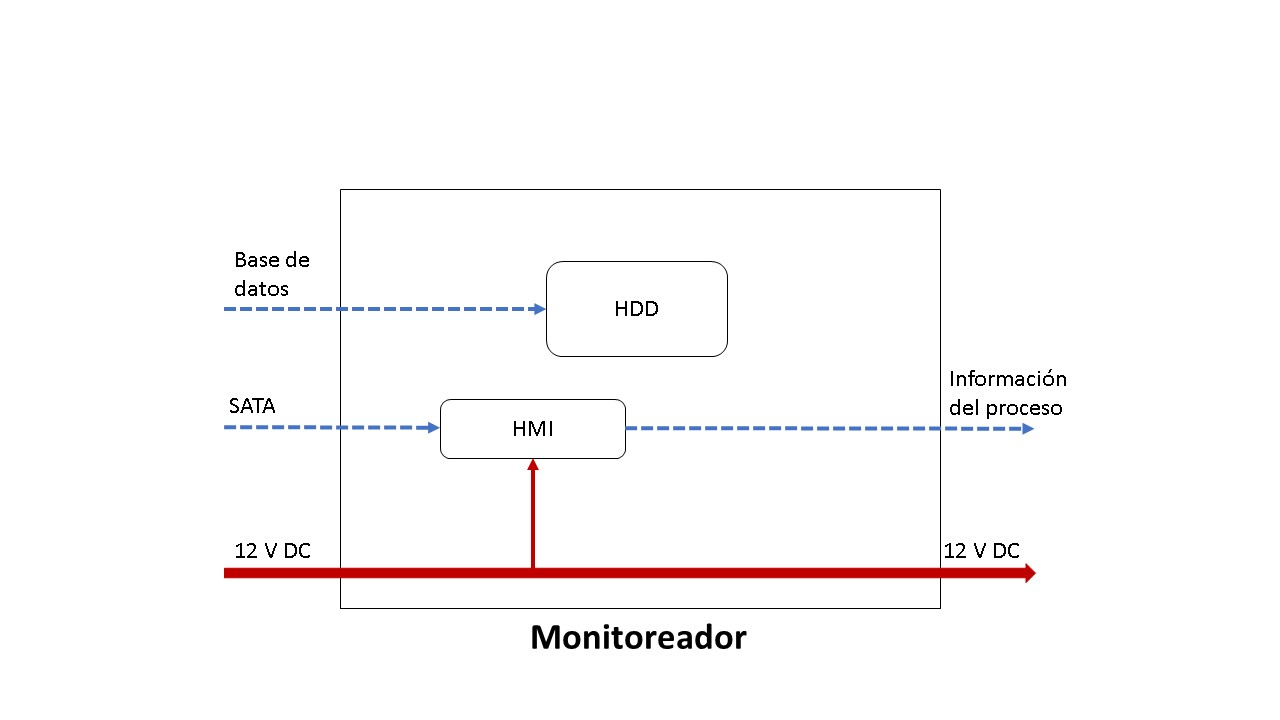
\includegraphics[scale=0.4]{Figuras/Monitoreador}
	\caption{Diagrama de bloques alimentación}
	\label{fig:DBAlimentacion}
\end{figure}

\chapterend{}